\documentclass{standalone}
\usepackage{tikz}
\usepackage{ctex,siunitx}
\setCJKmainfont{Noto Serif CJK SC}
\usepackage{tkz-euclide}
\usepackage{amsmath}
\usetikzlibrary{patterns, calc,3d}
\usetikzlibrary {decorations.pathmorphing,decorations.pathreplacing,decorations.shapes}
\tikzset{label style/.append style={font=\small}}
\begin{document}
\small
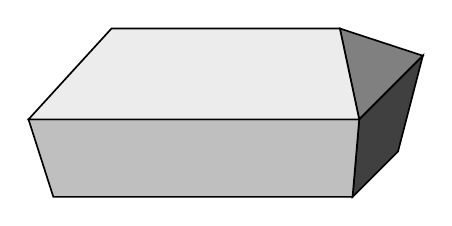
\begin{tikzpicture}[>=latex,scale=0.5,inner sep=1pt]
  \draw[semithick,fill=gray](4.2,2.2,2.1)--(2.9,3.7,0)--(4.2,2.2,-2.1)--cycle;
  \draw[semithick,fill=darkgray](4.2,2.2,-2.1)--(4.2,2.2,2.1)--(3.8,0,1.5)--(3.8,0,-1.5)--cycle;
  \draw[semithick,fill=lightgray](-3.8,0,1.5)--(3.8,0,1.5)--(4.2,2.2,2.1)--(-4.2,2.2,2.1)--cycle;
  \draw[semithick,fill=lightgray!30](-4.2,2.2,2.1)--(4.2,2.2,2.1)--(2.9,3.7,0)--(-2.9,3.7,0)--cycle;
\end{tikzpicture}
\end{document}